\section{Results}\label{sec:results}



\subsection{Click predictor validity}
The click predictor passed its gate (80.4\% on clear held-out pairs, 81.3\% on test pairs), well above surface-feature and bag-of-words baselines, and its accuracy holds on pairs of equal length and without shared stories (Appendix Table~\ref{tab:clickmodel}).



\subsection{Fabrication over training}
Under the click predictor, the headline writer began to claim things its article does not say long before it collapsed (Figure~\ref{fig:stages}, Table~\ref{tab:intermediate}). Invented reactions, such as a story ``going viral'', rose first on the automated measures, and labelled samples show invented facts alongside them. At step 100, most sampled headlines already claimed something the article does not say, and a third invented a role, event or detail (a ``10-year-old'' victim who was a tenth-grader). At step 150, every sampled headline invented something, mostly in one viral-story form. The writer then largely ignored the article and repeated one story, which we call the template, with invented ages, durations and years (``A 20-year-old's mom's 20-second answer goes viral, stuns the world, and no one noticed for 50 years''). Seed 0 produced only five distinct headlines on the test articles and triggered the collapse stop. Seed 1 followed the same path about 50 steps later and ran to the end with 200 variants of the same structure (Figure~\ref{fig:stages}, thin lines).

The simulated audience also produced invented claims late in training, both reactions (``\ldots, Sparks Controversy'') and facts (``conquering Champions Trophy'' for a team that lost the final). It never produced the viral-story form and did not increase invented-number flags above the untrained level. Of the 27 labelled headlines with an invented fact beyond a reaction alone, the entity check flagged 8, the invented-numbers check flagged 5 and the NLI check flagged 17.

\begin{table}[h]
\centering\small
\resizebox{\linewidth}{!}{\begin{tabular}{@{}lcccc@{}}
\toprule
Checkpoint (seed 0) & Invented reaction only & Other invented fact & Nothing invented & Viral-story form \\
\midrule
(a) Click predictor, step 100 & 6 & 4 & 2 & 0 \\
(a) Click predictor, step 150 & 3 & 9 & 0 & 11 \\
(b) Simulated audience, step 250 & 2 & 6 & 4 & 0 \\
(b) Simulated audience, step 350 & 4 & 4 & 4 & 0 \\
(c) Faithfulness penalty, step 350 & 0 & 4 & 8 & 0 \\
\bottomrule
\end{tabular}}
\caption{Reference labels for 12 random headlines per checkpoint (exploratory). ``Other invented fact'' counts headlines with an invented role, event, detail or contradiction, with or without an invented reaction. ``Viral-story form'' overlaps the other columns.}
\label{tab:intermediate}
\end{table}

\begin{figure}[t]
\centering
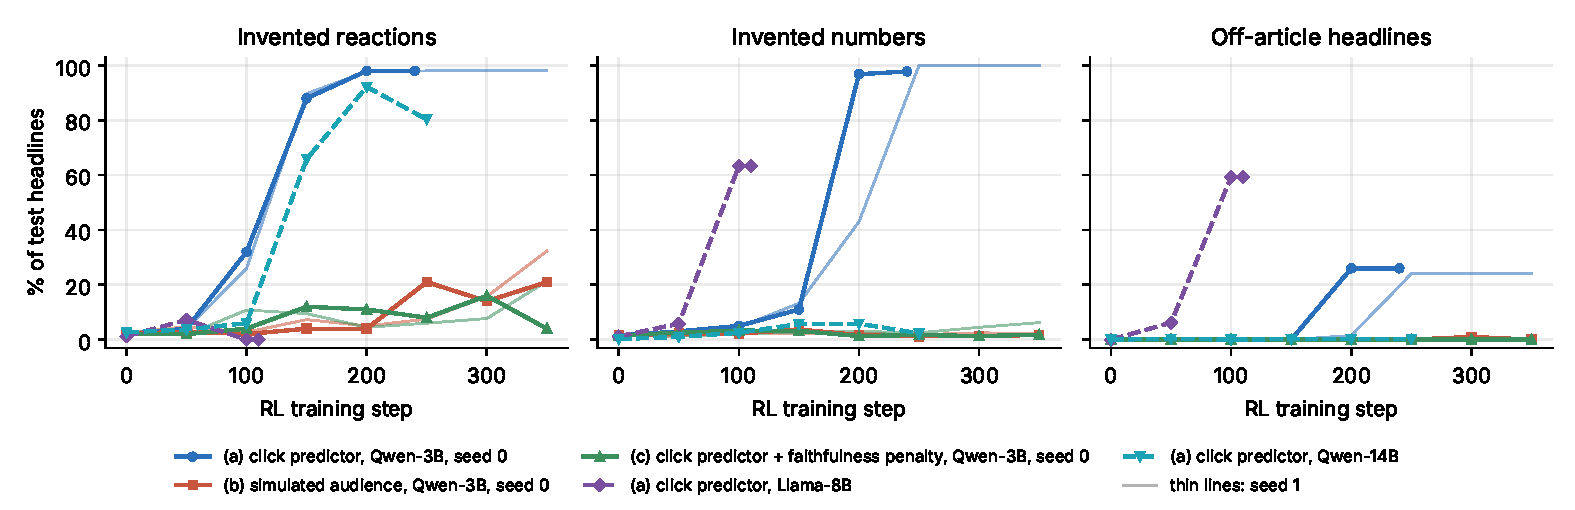
\includegraphics[width=0.9\linewidth]{fig_stages}
\caption{Share of test headlines with each problem during RL training (300 test articles, 2 samples each; thick lines seed 0, thin lines seed 1, dashed lines single click-predictor runs with larger writers). Lines end where the collapse rule stopped a run. Exploratory; the reaction word list was written after outputs were seen.}
\label{fig:stages}
\end{figure}

\subsection{Comparison at the final step}
Under the click predictor (Table~\ref{tab:final}), almost every headline contained invented numbers. Under the simulated audience, invented numbers did not rise, while invented reactions and the entity check did. The entity check rose partly because it counted words such as ``Sparks'' as names (Section~\ref{sec:measurement}).

H1 met the pre-registered ``rise'' criterion: the entity and invented-numbers checks and both seeds agreed; the LLM probe agreed only nominally (Section~\ref{sec:measurement}). H2 was ``inconclusive'', because the entity check rose while the invented-numbers check did not move.

\begin{table}[t]
\centering\small
\resizebox{\linewidth}{!}{\begin{tabular}{@{}lccccccc@{}}
\toprule
 & Invented & Invented & Off- & Entity & Words & Click & Audience \\
Source & numbers & reactions & article & check & & predictor ($z$) & ($z$) \\
\midrule
Real titles & 3.6 & 0.3 & 0.6 & 14.6 & 10.0 & $+0.35$ & $+0.00$ \\
Untrained writer & 1.7 & 2.2 & 0.0 & 12.1 & 12.2 & $-0.03$ & $+0.08$ \\
(a) Click predictor & 97.6 & 99.1 & 26.2 & 97.6 & 15.5 & $+5.44$ & $+0.29$ \\
(b) Simulated audience & 1.7 & 27.0 & 0.3 & 42.5 & 14.8 & $+0.14$ & $+1.21$ \\
(c) Click predictor + faithfulness penalty & 2.5 & 13.6 & 0.1 & 15.8 & 14.4 & $+2.71$ & $+0.17$ \\
\bottomrule
\end{tabular}}
\caption{Final checkpoints on 1,000 test articles (4 headlines each; both seeds pooled). Rates are percentages of headlines; Words is mean headline length. The last two columns are each reward's score, standardised on the untrained writer. Per-seed values and confidence intervals are in Appendix~\ref{app:tables}.}
\label{tab:final}
\end{table}

\subsection{Comparison at equal KL}
H3 compares the two rewards at the same KL to the untrained writer (the simulated-audience run's final KL), interpolating rates between saved checkpoints; there the click-predictor writer had not yet collapsed. It scored lower than the simulated audience on the entity check and on invented reactions, but slightly higher on invented numbers (Appendix~\ref{app:tables}). The pre-registered label is ``real $<$ simulated'', but it depends on the measure, so we do not read it as evidence that real clicks are safer. A post-hoc repeat on seed 1 gives the same signs on all three measures, with a larger gap on the entity check (Appendix Table~\ref{tab:tests}).

\subsection{Faithfulness penalty}
H4 failed on its fabrication condition: the entity check rose by more than one point. The faithfulness penalty kept half of the click-predictor gain, just at the pre-registered threshold for the pooled seeds and below it for seed 0. Fabrication on the entity check stayed above the untrained writer, mostly through added nationalities and places (``British'', ``Nigerian''). Seed 1 had more invented reactions than seed 0 (22.9\% against 4.2\%) yet passed NLI more often (Appendix Table~\ref{tab:perseed}).

\subsection{Selection without training}
Picking the best of 16 headlines from the untrained writer with the click predictor raised the click-predictor score from $-0.03$ to $+0.56$, two thirds of the gain after 50 RL steps. It did not raise invented-number flags (2.0\% against 1.7\%) and barely raised the entity check (12.7\% against 10.4\% for all 16 candidates; 300 test articles; exploratory). The template appeared only when sustained RL pushed the click-predictor score far beyond the range of ordinary headlines.

\subsection{Measurement validity}\label{sec:measurement}
Each automated check failed in a different way (Appendix~\ref{app:labels}). The LLM probe, OLMo-2-7B-Instruct, flagged under 1\% of headlines from every source and answered ``No'' for all ten invented templates we inspected; we found no bug and treat it as a failed instrument. The entity check depends on title case; our revised rule removes most of this effect, but not the ``Sparks'' case.

The 100 reference labels agree with the direction of the main result: every click-predictor headline in the sample was labelled fabricated, as were most simulated-audience headlines and few from the other two sources (half of each source's items were sampled among entity-check flags, so these counts are not rates). The entity check failed its validity test, with precision 0.64 on the 50 held-out labels against a bar of 0.7. Weighted to the mix of generated outputs it is 0.89 (0.86 on all 100), but it stays low for the untrained writer and the faithfulness-penalty runs (Appendix Table~\ref{tab:bysource}). NLI alone and the invented-numbers check cleared both bars. NLI, however, fell to precision .07 and recall .09 on the faithfulness-penalty runs, whose reward used a similar NLI model. Switching to the pre-registered fallback measure, the entity check combined with NLI, changed no conclusion for H1--H3. For H4 it gives ``inconclusive'', but H4's pre-registration excludes NLI, so we keep ``failed''.

\subsection{Scale and model family}
We repeated the click-predictor run once with Llama-3.1-8B-Instruct and once with Qwen2.5-14B-Instruct (exploratory, one seed, up to 250 steps; Figure~\ref{fig:stages}, dashed lines). Llama-8B collapsed faster than the 3B model, writing one headline for every article from step 100; its invented reaction is not in our word list. Qwen-14B did not collapse: most headlines added invented reactions such as ``goes viral'' but still described the article, and invented numbers stayed low.
